% \subsection{結果}
% \subsubsection{客観評価1: ベースラインと提案手法の比較}
% \label{sec4:sec:obj_1}
% 本節では,ベースラインと提案手法の比較を行う.比較手法は,以下の五つである.
% \begin{enumerate}
%     \item ベースライン
%     \item ネットワークA
%     \item ネットワークB(Not-Pretrained)
%     \item ネットワークC(Not-Pretrained)
%     \item ネットワークB(Pretrained)
%     \item ネットワークC(Pretrained)
% \end{enumerate}
% ベースラインは,提案手法(図\ref{sec4:fig:network})におけるネットワークAで,メルスペクトログラムとHuBERT離散特徴量を予測するマルチタスク学習手法である.ネットワークAは提案手法において,ネットワークBおよびCに入力を与える役割を果たすネットワークである.提案手法自体ではないが,その構成要素とはなっているため,ここでも客観評価指標を確認することとした.ネットワークB(Not-Pretrained)は,HuBERT Transformer層で事前学習済み重みを読み込まなかった場合のネットワークBである.これに関連して,ネットワークC(Not-Pretrained)はネットワークB(Not-Pretrained)を利用したネットワークCである.これらに対し,ネットワークB(Pretrained)およびネットワークC(Pretrained)は,ネットワークBの学習時にHuBERT Transformer層で事前学習済み重みを読み込んだ点のみ異なる.

% まず,損失関数~\eqref{sec4:eq:loss}の重み係数$\lambda_{ssl^{d}}$を変化させた時の,客観評価指標の全テストデータに渡る平均値を表~\ref{sec4:tab:obj_weights}に示す.各手法ごとに$\lambda_{ssl^{d}}$を0.0001から1.0まで,10倍刻みで5段階検討するグリッドサーチを行い,各手法の客観評価指標ごとに,最も優れた値を下線で示している.ここで,提案手法ではネットワークAを学習し,その後Aを固定してBを学習し,最後にAとBを固定してCを学習するように実装している.これに対し,$\lambda_{ssl}^{d}$のグリッドサーチでは,この一連の流れに対して一つの値を検討した.例えば,ネットワークB(Not-Pretrained)で$\lambda_{ssl^{d}}$が0.0001の場合,ネットワークAには$\lambda_{ssl^{d}}$が0.0001の場合を用いている.ネットワークC(Not-Pretrained)で$\lambda_{ssl^{d}}$が0.0001の場合,ネットワークA,Bともに$\lambda_{ssl^{d}}$が0.0001の場合を用いている.また,この後手法ごとの比較を行う際には,各手法ごとにグリッドサーチで得られた最適な場合同士を比較するため,最適だと判断した場合を太字で示している.

% \begin{table*}[bt]
%     \centering
%     \caption{損失関数の重み係数$\lambda_{ssl^{d}}$による客観評価指標の比較}
%     \label{sec4:tab:obj_weights}
%     \begin{center}
%         \renewcommand{\arraystretch}{1.0} % 行の高さ調整
%         \setlength{\tabcolsep}{8pt}      % 列の幅調整
%         \scalebox{1.0}{
%             \begin{tabular}{|c|l|rr|}
%                 \hline
%                 \multicolumn{1}{|c|}{手法}         & \multicolumn{1}{c|}{$\lambda_{ssl^{d}}$} & \multicolumn{1}{c}{WER [\%]} & \multicolumn{1}{c|}{話者類似度} \\
%                 \hline
%                 ベースライン                           & 0.0001                                   & 57.3                         & 0.833                      \\
%                 \textbf{ベースライン}                  & \textbf{0.001}                           & \underline{\textbf{54.6}}    & \textbf{0.836}             \\
%                 ベースライン                           & 0.01                                     & 56.2                         & \underline{0.837}          \\
%                 ベースライン                           & 0.1                                      & 58.2                         & 0.784                      \\
%                 ベースライン                           & 1                                        & 59.0                         & 0.685                      \\
%                 \hline
%                 ネットワークA                          & 0.0001                                   & 55.4                         & 0.841                      \\
%                 ネットワークA                          & 0.001                                    & 55.1                         & 0.842                      \\
%                 ネットワークA                          & 0.01                                     & \underline{53.4}             & \underline{0.843}          \\
%                 ネットワークA                          & 0.1                                      & 54.6                         & 0.809                      \\
%                 ネットワークA                          & 1                                        & 58.7                         & 0.698                      \\
%                 \hline
%                 ネットワークB(Not-Pretrained)          & 0.0001                                   & 60.6                         & \underline{0.852}          \\
%                 ネットワークB(Not-Pretrained)          & 0.001                                    & 56.7                         & 0.829                      \\
%                 ネットワークB(Not-Pretrained)          & 0.01                                     & 54.4                         & 0.847                      \\
%                 \textbf{ネットワークB(Not-Pretrained)} & \textbf{0.1}                             & \underline{\textbf{45.3}}    & \textbf{0.840}             \\
%                 ネットワークB(Not-Pretrained)          & 1                                        & 45.5                         & 0.712                      \\
%                 \hline
%                 ネットワークC(Not-Pretrained)          & 0.0001                                   & 58.5                         & \underline{0.860}          \\
%                 ネットワークC(Not-Pretrained)          & 0.001                                    & 55.0                         & 0.850                      \\
%                 ネットワークC(Not-Pretrained)          & 0.01                                     & 56.0                         & 0.848                      \\
%                 \textbf{ネットワークC(Not-Pretrained)} & \textbf{0.1}                             & \underline{\textbf{45.8}}    & \textbf{0.848}             \\
%                 ネットワークC(Not-Pretrained)          & 1                                        & 46.9                         & 0.763                      \\
%                 \hline
%                 ネットワークB(Pretrained)              & 0.0001                                   & 60.1                         & 0.841                      \\
%                 ネットワークB(Pretrained)              & 0.001                                    & 57.1                         & 0.839                      \\
%                 ネットワークB(Pretrained)              & 0.01                                     & 56.8                         & \underline{0.860}          \\
%                 \textbf{ネットワークB(Pretrained)}     & \textbf{0.1}                             & \underline{\textbf{44.2}}    & \textbf{0.778}             \\
%                 ネットワークB(Pretrained)              & 1                                        & 48.1                         & 0.685                      \\
%                 \hline
%                 ネットワークC(Pretrained)              & 0.0001                                   & 57.8                         & 0.861                      \\
%                 ネットワークC(Pretrained)              & 0.001                                    & 57.2                         & 0.865                      \\
%                 ネットワークC(Pretrained)              & 0.01                                     & 55.7                         & \underline{0.870}          \\
%                 \textbf{ネットワークC(Pretrained)}     & \textbf{0.1}                             & \underline{\textbf{45.5}}    & \textbf{0.849}             \\
%                 ネットワークC(Pretrained)              & 1                                        & 46.2                         & 0.753                      \\
%                 \hline
%             \end{tabular}
%         }
%     \end{center}
% \end{table*}

% \begin{figure}[bt]
%     \centering
%     \begin{subfigure}{\linewidth}
%         \centering
%         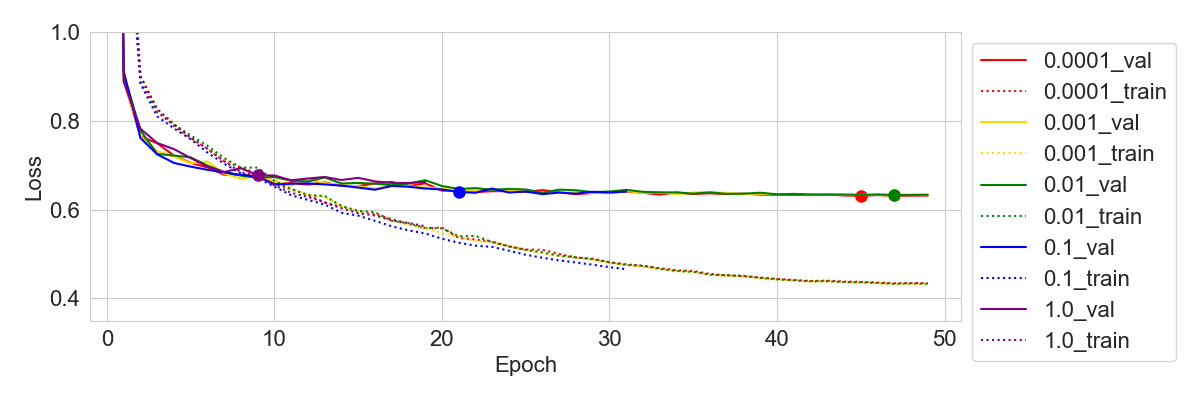
\includegraphics[height=55mm]{./figure/sec4/learning_curves/0/mel_loss.png}
%         \caption{メルスペクトログラムのMAE Loss(式~\eqref{sec4:eq:loss}の$L_{mel}$)}
%         \label{sec4:fig:learning_curve_baseline_val_mel_loss}
%     \end{subfigure}
%     \begin{subfigure}{\linewidth}
%         \centering
%         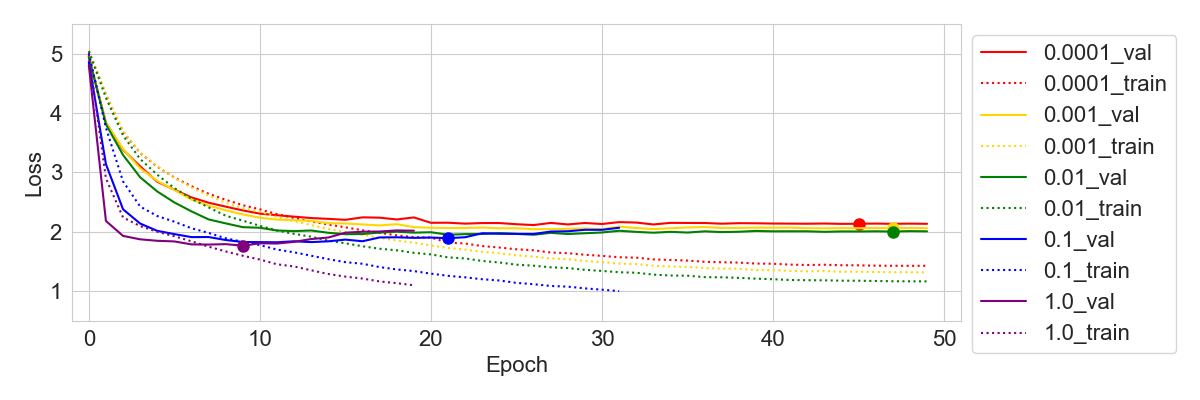
\includegraphics[height=55mm]{./figure/sec4/learning_curves/0/ssl_feature_cluster_loss.png}
%         \caption{HuBERT離散特徴量のCross Entropy Loss(式~\eqref{sec4:eq:loss}の$L_{ssl^{d}}$)}
%         \label{sec4:fig:learning_curve_baseline_val_ssl_feature_cluster_loss}
%     \end{subfigure}
%     \begin{subfigure}{\linewidth}
%         \centering
%         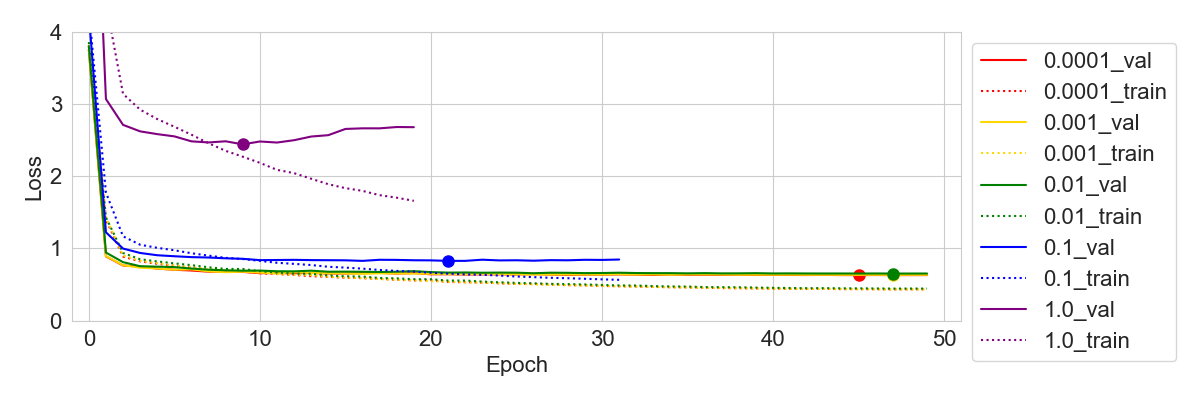
\includegraphics[height=55mm]{./figure/sec4/learning_curves/0/total_loss.png}
%         \caption{損失の合計値(式~\eqref{sec4:eq:loss}の$L$)}
%         \label{sec4:fig:learning_curve_baseline_val_total_loss}
%     \end{subfigure}
%     \caption{ベースラインにおける学習曲線}
%     \label{sec4:fig:learning_curve_baseline_val_losses}
% \end{figure}

% \begin{figure}[bt]
%     \centering
%     \begin{subfigure}{\linewidth}
%         \centering
%         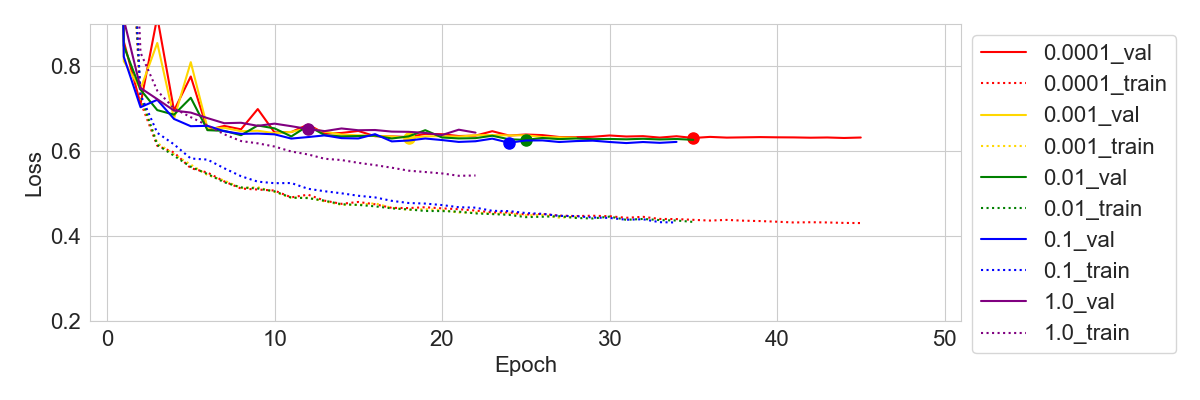
\includegraphics[height=55mm]{./figure/sec4/learning_curves/2/mel_loss.png}
%         \caption{メルスペクトログラムのMAE Loss(式~\eqref{sec4:eq:loss}の$L_{mel}$)}
%         \label{sec4:fig:learning_curve_method_2_val_mel_loss}
%     \end{subfigure}
%     \begin{subfigure}{\linewidth}
%         \centering
%         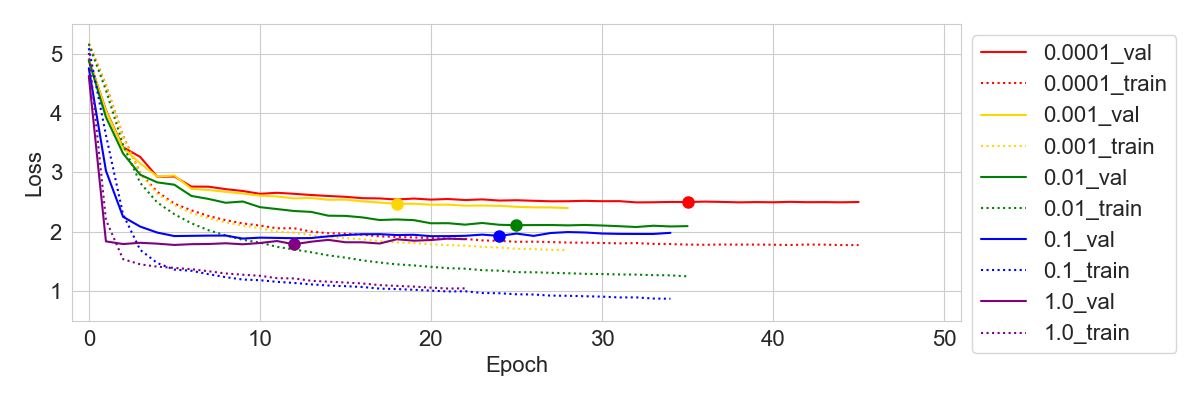
\includegraphics[height=55mm]{./figure/sec4/learning_curves/2/ssl_feature_cluster_loss.png}
%         \caption{HuBERT離散特徴量のCross Entropy Loss(式~\eqref{sec4:eq:loss}の$L_{ssl^{d}}$)}
%         \label{sec4:fig:learning_curve_method_2_val_ssl_feature_cluster_loss}
%     \end{subfigure}
%     \begin{subfigure}{\linewidth}
%         \centering
%         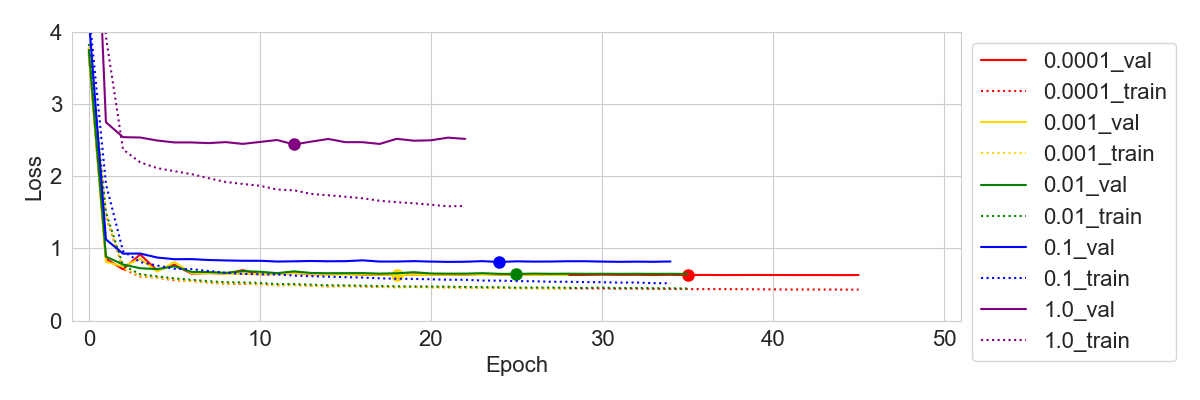
\includegraphics[height=55mm]{./figure/sec4/learning_curves/2/total_loss.png}
%         \caption{損失の合計値(式~\eqref{sec4:eq:loss}の$L$)}
%         \label{sec4:fig:learning_curve_method_2_val_total_loss}
%     \end{subfigure}
%     \caption{ネットワークB(Not-Pretrained)における学習曲線}
%     \label{sec4:fig:learning_curve_method_2_val_losses}
% \end{figure}

% ベースラインでは,$\lambda_{ssl^{d}}$の値が0.001のときにWERが最も低く,0.01のときに話者類似度が最も高くなった.現状WERの高さが特に課題であり,話者類似度はほとんど同じであったため,今回は0.001が最適であると判断した.次に,図~\ref{sec4:fig:learning_curve_baseline_val_losses}にベースラインにおける学習曲線の結果を示す.横軸がエポック数,縦軸が損失の値を表す.損失の値は各エポックにおける平均値である.実線は検証データに対する損失,点線は学習データに対する損失を表しており,線の色は$\lambda_{ssl^{d}}$の違いを表す.また,丸いマーカーは表~\ref{sec4:tab:obj_method_comp}に示した最良エポック時における検証データに対する損失の値を表す.学習曲線より,$\lambda_{ssl^{d}}$の値を変化させることによって,特に$L_{ssl^{d}}$の傾向が変化していることがわかる.具体的には,$\lambda_{ssl^{d}}$の値を0.0001から1.0へと増加させるのに伴って,学習初期における損失の下がり方が急峻になっており,達する最小値自体が小さくなっていることがわかる.また,$\lambda_{ssl^{d}}$の値が0.1以上の場合,検証データに対する$L_{ssl^{d}}$は早いうちから増加傾向に転じている.これに伴い,今回は検証データに対する$L$の値を監視し,Early Stoppingの適用と最良エポックの決定を行なったため,$L_{mel}$が下がり切らない状態で学習が中断される結果となった.離散化して冗長性を排除したHuBERT離散特徴量と比較して,メルスペクトログラムが特に話者性を反映するために必要な特徴量だと考えられるため,$\lambda_{ssl^{d}}$が0.1以上の場合に見られた話者類似度の顕著な低下は,$L_{mel}$を下げきれなかったことが原因だと考えられる.

% ネットワークAでは,提案手法の構成要素であるため,特に最適な手法の選択は行なっていない.ベースラインとの違いは$L_{ssl^{i}}$が損失に含まれることであるが,客観評価指標より,ベースラインと性能は概ね同等であることがわかる.学習曲線の傾向については,ベースラインと同様であったため省略する.

% ネットワークB(Not-Pretrained)では,$\lambda_{ssl^{d}}$の値が0.1の時にWERが最も低く,0.0001の時に話者類似度が最も高くなった.ここではWERの低さを優先し,0.1が最適だと判断した.次に,図~\ref{sec4:fig:learning_curve_method_2_val_losses}にネットワークB(Not-Pretrained)における学習曲線の結果を示す.ベースラインと同様に,$\lambda_{ssl^{d}}$の値を0.0001から1.0へと増加させるのに伴って,学習初期における$L_{ssl^{d}}$の下がり方が急峻になっており,達する最小値自体が小さくなっていることがわかる.また,$\lambda_{ssl^{d}}$が1.0の場合に$L_{mel}$を下げきれなくなる傾向が見られ,ベースラインと同様にこのとき話者類似度の顕著な低下が確認された.加えて,ネットワークB(Not-Pretrained)では$\lambda_{ssl^{d}}$が0.1の場合における$L_{ssl^{d}}$の増加が緩やかであり,$L_{mel}$も十分下げられていることがわかる.さらに,$\lambda_{ssl^{d}}$が0.1の場合,$L_{mel}$の達する最小値自体が,$\lambda_{ssl^{d}}$が0.01以下の場合と比較して小さくなっていることがわかる.これはベースラインでは見られなかった新たな傾向であった.最適な$\lambda_{ssl^{d}}$の値は客観評価指標から0.1としたが,学習曲線の挙動より,この時他の値の場合と比較して$L_{mel}$と$L_{ssl^{d}}$の両方をバランスよく下げられていたと言える.

% ネットワークC(Not-Pretrained)では,$\lambda_{ssl^{d}}$が0.1の場合が最適だと判断した.判断理由はネットワークB(Not-Pretrained)と同様である.学習曲線の傾向については,ネットワークB(Not-Pretrained)と同様であったため省略する.

% ネットワークB(Pretrained)では,$\lambda_{ssl^{d}}$を0.1としたときにWERが最低となる一方で,0.01以上の場合と比較したときの話者類似度の低下が顕著であり,事前学習済み重みを読み込まなかったネットワークB(Not-Pretrained)とは異なる傾向であった.今回はWERが低いことを優先して,0.1が最適であると判断した.学習曲線の傾向については,ネットワークB(Not-Pretrained)と同様であったため省略する.学習曲線が同様であるにも関わらず結果の傾向が異なったことについては,重みの初期値が異なっていれば損失の値が同様だとしても異なる局所最適解に収束する可能性があるため,妥当だと判断した.

% ネットワークC(Pretrained)では,$\lambda_{ssl^{d}}$の値が0.1の時にWERが最も低く,0.01の時に話者類似度が最も高くなった.ここでもWERが最低であることを優先して,0.1が最適だと判断した.学習曲線の傾向はネットワークB(Not-Pretrained)と同様であったため省略する.

% 次に,最適なチューニングをした場合における,手法ごとの客観評価指標の全テストデータに渡る平均値を表~\ref{sec4:tab:obj_method_comp}に示す.分析合成は,原音声から計算した特徴量を入力として,Multi-input Vocoderで逆変換した合成音声であり,本実験下において合成音声により達成され得る上限値を表す.ベースラインからネットワークC(Pretrained)については,表~\ref{sec4:tab:obj_weights}において太字としたもの,すなわち最適なチューニングだと判断されたものを選択している.また,ベースラインからネットワークC(Pretrained)の中で,最も優れた値を下線で示している.これより,提案手法であるネットワークB(Not-Pretrained),ネットワークC(Not-Pretrained),ネットワークC(Pretrained)の三つは,ベースラインに対してWERと話者類似度の両方を改善したことがわかる.一方,ネットワークB(Pretrained)はWERの改善を達成したが,話者類似度については悪化したことがわかる.ここで,HuBERTの事前学習済み重みを初期値とすることの効果について,ネットワークB(Not-Pretrained)とネットワークB(Pretrained)を比較すると,ネットワークB(Pretrained)の方がWERは1.1\%低いが,話者類似度も0.062低いことがわかる.実際に音声を聞いてみると,音声に不自然なノイズが含まれており,原音声に対する類似性が下がっていることが確認された.よって,HuBERTの事前学習済み重みを初期値としたHuBERT Transformer層の転移学習は,本タスクにおいて有効でないと考えられる.また,ネットワークCの導入効果について,ネットワークB(Not-Pretrained)とネットワークC(Not-Pretrained)を比較すると,ほとんど結果が変わらないことがわかる.一方,ネットワークB(Pretrained)とネットワークC(Pretrained)を比較すると,特に話者類似度についてネットワークC(Pretrained)はネットワークB(Pretrained)よりも0.071高いことがわかる.これより,ネットワークCの効果は,ベースとなるネットワークBの性能に依存して変化すると考えられる.

% \begin{table*}[bt]
%     \centering
%     \caption{最適なチューニングをした場合における手法ごとの比較}
%     \label{sec4:tab:obj_method_comp}
%     \begin{center}
%         \renewcommand{\arraystretch}{1.0} % 行の高さ調整
%         \setlength{\tabcolsep}{8pt}      % 列の幅調整
%         \scalebox{1.0}{
%             \begin{tabular}{|c|l|rr|}
%                 \hline
%                 \multicolumn{1}{|c|}{手法} & \multicolumn{1}{c|}{$\lambda_{ssl^{d}}$} & \multicolumn{1}{c}{WER [\%]} & \multicolumn{1}{c|}{話者類似度} \\
%                 \hline
%                 ベースライン                   & 0.001                                    & 54.6                         & 0.836                      \\
%                 ネットワークB(Not-Pretrained)  & 0.1                                      & 45.3                         & 0.840                      \\
%                 ネットワークC(Not-Pretrained)  & 0.1                                      & 45.8                         & 0.848                      \\
%                 ネットワークB(Pretrained)      & 0.1                                      & \underline{44.2}             & 0.778                      \\
%                 ネットワークC(Pretrained)      & 0.1                                      & 45.5                         & \underline{0.849}          \\
%                 \hline
%                 分析合成                     & \multicolumn{1}{c|}{-}                   & 3.7                          & 0.956                      \\
%                 原音声                      & \multicolumn{1}{c|}{-}                   & 3.7                          & 1.000                      \\
%                 \hline
%             \end{tabular}
%         }
%     \end{center}
% \end{table*}

% \subsubsection{客観評価2: 提案手法のさらなる検討}
% \label{sec4:sec:obj_2}
% 本節では,\ref{sec4:sec:obj_1}節の客観評価によって得られた知見をもとに,さらなる提案手法の検討を行った結果を述べる.まず,\ref{sec4:sec:obj_1}節より,これまでに検討した提案手法の中で最も優れているのはネットワークB(Not-Pretrained)だと判断した.選択理由について,まずネットワークC(Not-Pretrained)とネットワークB(Not-Pretrained)はほとんど差がないため,ネットワークCの導入効果はほとんどないと判断しネットワークC(Not-Pretrained)を省いた.次に,ネットワークB(Pretrained)はネットワークB(Not-Pretrained)と比較してWERは1.2\%低いがその差は小さく,一方で話者類似度では顕著な低下が見られた.よって,ネットワークB(Pretrained)は本実験下においては効果的でないと判断した.最後に,ネットワークC(Pretrained)について,客観評価指標の値はネットワークB(Not-Pretrained)と同等であり,元となっているネットワークB(Pretrained)を省いたことも考慮して,ネットワークC(Pretrained)も省くこととした.

% ネットワークB(Not-Pretrained)に対し,まずはHuBERT Transformer層への入力特徴量について検討した.\ref{sec4:sec:obj_1}節では事前学習済み重みを用いることの有効性を調べる目的があったため,入力は事前学習時に揃えてHuBERT中間特徴量としていた.しかし,選択したネットワークB(Not-Pretrained)は事前学習済み重みを利用しないため,HuBERT中間特徴量を入力とすることが意味をなしているか不明である.これに対し,今回はネットワークAからマルチタスク学習によって同時に予測される,メルスペクトログラムとHuBERT離散特徴量を入力とする場合を比較した.入力の際,メルスペクトログラムは連続したフレームをチャンネル方向に積んで,100Hz・80次元から50Hz・160次元に形状を変換した.HuBERT離散特徴量は,モデルから出力される予測確率分布をそのまま利用した.HiFi-GAN入力のように,一度トークンに変換してからベクトル表現を得るという手段も考えられたが,トークンに変換するためには予測確率を元にトークンをサンプリングする必要があり,これは微分不可能な操作であるため学習が不可能となる.そのため,ここでは予測確率分布をそのまま特徴量として利用することにした.パディング部のトークンを含むため,予測確率分布の次元は101次元である.これらを結合して$160 + 101 = 261$次元の特徴量とした上で,全結合層を通してHuBERT中間特徴量と同じ768次元までチャンネル数を上げ,HuBERT Transformer層への入力とした.これまでと同様に,五種類の$\lambda_{ssl^{d}}$でグリッドサーチを行った結果を表\ref{sec4:tab:obj_weights_networkb_input_comparison}に示す.新たに検討した手法はネットワークB(Not-Pretrained・Mel-Hub)とした.客観評価指標ごとに最も優れた値を下線で示しており,ネットワークB(Not-Pretrained・Mel-Hub)については最適だと判断した場合を太字で示している.これより,ネットワークB(Not-Pretrained・Mel-Hub)では,ネットワークB(Not-Pretrained)で見られたようなWERが下がる重みが確認されないことがわかる.最適だと判断した$\lambda_{ssl^{d}}$が0.001の場合においても,話者類似度はネットワークB(Not-Pretrained)よりも0.005とわずかに高いが,WERは10.1\%高い.これより,ネットワークB(Not-Pretrained・Mel-Hub)は,ネットワークB(Not-Pretrained)に劣ると判断した.この結果より,HuBERT中間特徴量はメルスペクトログラムとHuBERT離散特徴量の複合特徴量と比較して,ネットワークBの推定精度改善につながるより良い入力特徴量であったと考えられる.HuBERT中間特徴量は768次元であったのに対し,メルスペクトログラムとHuBERT離散特徴量の複合特徴量は261次元であるから,より高次元で冗長性が高い方が,ネットワークBによる特徴抽出の対象として優れていたのではないかと考える.

% \begin{table*}[bt]
%     \centering
%     \caption{HuBERT Transformer層への入力特徴量を変化させた場合の比較}
%     \label{sec4:tab:obj_weights_networkb_input_comparison}
%     \begin{center}
%         \renewcommand{\arraystretch}{1.0} % 行の高さ調整
%         \setlength{\tabcolsep}{8pt}      % 列の幅調整
%         \scalebox{0.98}{
%             \begin{tabular}{|c|l|rr|}
%                 \hline
%                 \multicolumn{1}{|c|}{手法}                 & \multicolumn{1}{c|}{$\lambda_{ssl^{d}}$} & \multicolumn{1}{c}{WER [\%]} & \multicolumn{1}{c|}{話者類似度} \\
%                 \hline
%                 ネットワークB(Not-Pretrained・Mel-HuB)          & 0.0001                                   & 59.5                         & 0.840                      \\
%                 \textbf{ネットワークB(Not-Pretrained・Mel-HuB)} & \textbf{0.001}                           & \textbf{55.4}                & \underline{\textbf{0.845}} \\
%                 ネットワークB(Not-Pretrained・Mel-HuB)          & 0.01                                     & 56.2                         & 0.803                      \\
%                 ネットワークB(Not-Pretrained・Mel-HuB)          & 0.1                                      & 57.7                         & 0.795                      \\
%                 ネットワークB(Not-Pretrained・Mel-HuB)          & 1                                        & 58.1                         & 0.711                      \\
%                 \hline
%                 ネットワークB(Not-Pretrained)                  & 0.1                                      & \underline{45.3}             & 0.840                      \\
%                 \hline
%             \end{tabular}
%         }
%     \end{center}
% \end{table*}

% 次に,HuBERT中間特徴量をネットワークBに与えている,ネットワークAの学習方法を検討した.これまでの提案手法では,先行研究\cite{kim2023lip_multitask, choi2023intelligible}において報告されたマルチタスク学習の有効性を考慮し,ネットワークAにおいてHuBERT中間特徴量だけでなく,メルスペクトログラム,HuBERT離散特徴量を同時に予測するマルチタスク学習を採用していた.これに対し,ネットワークAにおいてHuBERT中間特徴量のみを推定するよう学習する場合を検討することで,マルチタスク学習の有効性を調べた.結果を表\ref{sec4:tab:obj_weights_networka_multitask}に示す.新たに検討した手法はネットワークB(Not-Pretrained・A-SingleTask)とした.客観評価指標ごとに最も優れた値を下線で示しており,ネットワークB(Not-Pretrained・A-SingleTask)については最適だと判断した場合を太字で示している.これより,ネットワークB(Not-Pretrained・A-SingleTask)で最適な場合を見ると,ネットワークB(Not-Pretrained)よりもWERが2.8\%低く,話者類似度は0.007高いことがわかる.従って,ネットワークAではネットワークBの入力に必要なHuBERT中間特徴量のみを推定する方が,メルスペクトログラムとHuBERT離散特徴量を同時に予測するマルチタスク学習を行うよりも,ネットワークBにより良い入力特徴量を与えられると考えられる.マルチタスク学習を行う場合,メルスペクトログラムやHuBERT離散特徴量が損失に加わるため,それらの損失を小さくするための勾配も考慮した重みの更新が行われるが,これがネットワークBに入力するHuBERT中間特徴量を推定する上では,悪影響を与えていると考えられる.

% \begin{table*}[bt]
%     \centering
%     \caption{ネットワークAにおけるマルチタスク学習の有無による比較}
%     \label{sec4:tab:obj_weights_networka_multitask}
%     \begin{center}
%         \renewcommand{\arraystretch}{1.0} % 行の高さ調整
%         \setlength{\tabcolsep}{8pt}      % 列の幅調整
%         \scalebox{0.96}{
%             \begin{tabular}{|c|l|rr|}
%                 \hline
%                 \multicolumn{1}{|c|}{手法}                      & \multicolumn{1}{c|}{$\lambda_{ssl^{d}}$} & \multicolumn{1}{c}{WER [\%]} & \multicolumn{1}{c|}{話者類似度} \\
%                 \hline
%                 ネットワークB(Not-Pretrained・A-SingleTask)          & 0.0001                                   & 54.0                         & \underline{0.867}          \\
%                 ネットワークB(Not-Pretrained・A-SingleTask)          & 0.001                                    & 52.2                         & 0.865                      \\
%                 ネットワークB(Not-Pretrained・A-SingleTask)          & 0.01                                     & 51.8                         & 0.843                      \\
%                 \textbf{ネットワークB(Not-Pretrained・A-SingleTask)} & \textbf{0.1}                             & \underline{\textbf{42.5}}    & \textbf{0.847}             \\
%                 ネットワークB(Not-Pretrained・A-SingleTask)          & 1                                        & 43.0                         & 0.768                      \\
%                 \hline
%                 ネットワークB(Not-Pretrained)                       & 0.1                                      & 45.3                         & 0.840                      \\
%                 \hline
%             \end{tabular}
%         }
%     \end{center}
% \end{table*}

% \subsubsection{主観評価}
% 主観評価実験は,本実験で検討した提案手法がベースラインに対する改善を達成したか否かを確認するために行った.\ref{sec4:sec:obj_1}節および\ref{sec4:sec:obj_2}節の検討結果より,本研究の提案手法の代表としては,ネットワークB(Not-Pretrained)と,ネットワークB(Not-Pretrained・SingleTask)を選択した.なぜなら,客観評価指標の結果から,最良だと考えられる提案手法はネットワークB(Not-Pretrained・SingleTask)であるが,ネットワークB(Not-Pretrained)もそれに次ぐ性能であり,ネットワークAにおけるマルチタスク学習の有無が主観評価において有意な差であるかも確かめたいと考えたからである.結果として,主観評価実験において比較する音声は以下の五種類である.
% \begin{enumerate}
%     \item ベースライン
%     \item ネットワークB(Not-Pretrained)
%     \item ネットワークB(Not-Pretrained・A-SingleTask)
%     \item 分析合成
%     \item 原音声
% \end{enumerate}
% \ref{sec4:sec:sbj_explanation}節で述べたように,主観評価では音声の明瞭性と類似性を五段階評価した.総被験者数は75人としたが,アプリの不具合によるエラーを理由に一名のデータを除き,それ以外の被験者についてはダミーサンプルの回答が正しかったためそのまま用いて,74名分のデータで統計処理を実施した.被験者の年齢層は21歳から62歳に渡った.年齢層の箱ひげ図を図\ref{sec4:fig:age}に示す.被験者の性別は男性32名,女性42名であった.また,実験に利用した音響機器はヘッドホンが18名,イヤホンが56名であった.
% \begin{figure}[bt]
%     \centering
%     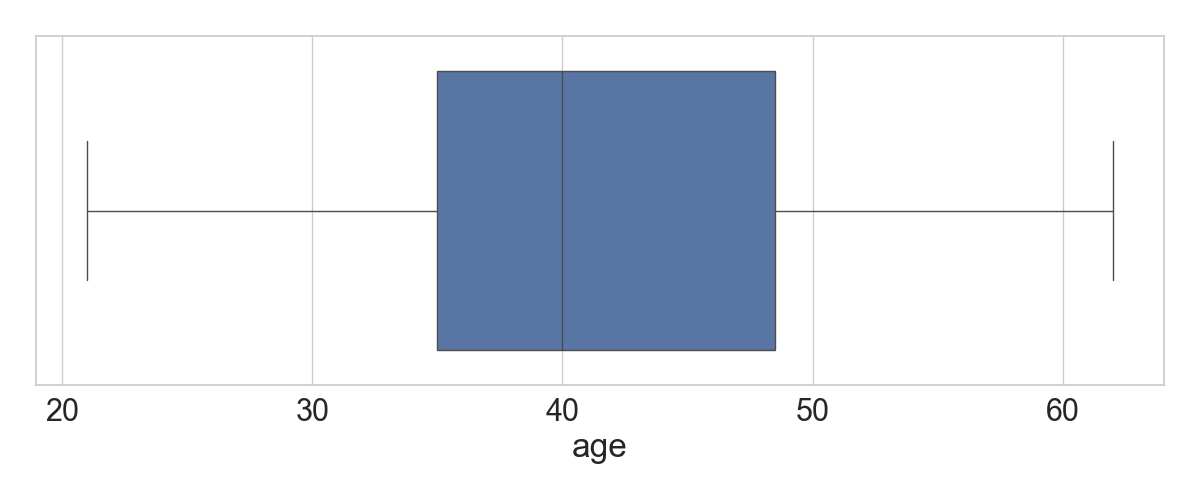
\includegraphics[height=50mm]{./figure/sec4/sbj/age.png}
%     \caption{主観評価実験における被験者の年齢層}
%     \label{sec4:fig:age}
% \end{figure}

% 明瞭性と類似性の評価値について,手法ごとに平均値と95\%信頼区間を計算した結果を表\ref{sec4:tab:sbj_mean_ci}に示す.また,各手法の組み合わせについて,平均値の差の検定(片側検定)を行った結果を表\ref{sec4:tab:sbj_int_p}, \ref{sec4:tab:sbj_sim_p}に示す.表における$\lr{i, j}$成分は,$i$行目の手法に対する評価値の母平均を$\mu_{i}$,$j$列目の手法に対する評価値の母平均を$\mu_{j}$とするとき,帰無仮説を$\mu_{i} = \mu_{j}$,対立仮説を$\mu_{i} > \mu_{j}$とした片側検定で計算されたp値に対し,Benjamini/Hochberg法による多重比較のための補正を行った結果である.ここで,表の文字列はそれぞれの以下の略称とする.
% \begin{enumerate}
%     \item GT: 原音声(Ground Truth)
%     \item AbS: 分析合成(Analysis by Synthesis)
%     \item B(N-P, A-S): ネットワークB(Not-Pretrained・A-SingleTask)
%     \item B(N-P): ネットワークB(Not-Pretrained)
%     \item Baseline: ベースライン
% \end{enumerate}
% また,本実験における有意水準は5\%とする.

% まず,表\ref{sec4:tab:sbj_int_p}より,提案したネットワークB(Not-Pretrained)およびネットワークB(Not-Pretrained・A-SingleTask)は,ベースラインに対して明瞭性の評価値が有意に高いことがわかる.これより,二つの提案手法はどちらもベースラインより話者の想定した発話内容を正確に反映した合成音声を実現できたと考えられる.一方,提案手法二つの間には有意差がないことも分かる.これより,ネットワークAの学習方法の違いは明瞭性に有意な差をもたらさなかったと言える.次に,表\ref{sec4:tab:sbj_sim_p}より,提案したネットワークB(Not-Pretrained)およびネットワークB(Not-Pretrained・A-SingleTask)は,ベースラインに対して類似性の評価値が有意に高いことがわかる.これより,二つの提案手法はどちらもベースラインより原音声に似た合成音声を実現できたと考えられる.また,ここでは提案手法二つの間にも有意差があることが分かる.これより,ネットワークAの学習方法の違いは明瞭性に有意な差をもたらさなかったが,類似性には有意な差をもたらしたと言える.

% 以上のことから,ネットワークB(Not-Pretrained・A-SingleTask)が明瞭性・類似性の両面において,最も優れた合成音声を実現したと考えられる.一方,ネットワークB(Not-Pretrained・A-SingleTask)と,合成音声の性能上限を表す分析合成の間には未だ大きな差があり,特に自然音声に迫る合成音の実現は達成されていない.従って,本実験におけるベースラインからの改善は達成したものの,今後もさらなるネットワークの改善が必要だと考えられる.

% \begin{table*}[bt]
%     \centering
%     \caption{主観評価実験の結果より計算した標本平均と95\%信頼区間}
%     \label{sec4:tab:sbj_mean_ci}
%     \begin{center}
%         \renewcommand{\arraystretch}{1.0} % 行の高さ調整
%         \setlength{\tabcolsep}{8pt}      % 列の幅調整
%         \scalebox{0.95}{
%             \begin{tabular}{|c|l|rr|}
%                 \hline
%                 \multicolumn{1}{|c|}{手法}             & \multicolumn{1}{c|}{$\lambda_{ssl^{d}}$} & \multicolumn{1}{c}{明瞭性} & \multicolumn{1}{c|}{類似性} \\
%                 \hline
%                 ベースライン                               & 0.001                                    & $2.371 \pm 0.072$       & $2.933 \pm 0.080$        \\
%                 ネットワークB(Not-Pretrained)              & 0.1                                      & $2.753 \pm 0.075$       & $3.052 \pm 0.085$        \\
%                 ネットワークB(Not-Pretrained・A-SingleTask) & 0.1                                      & $2.818 \pm 0.079$       & $3.182 \pm 0.082$        \\
%                 \hline
%                 分析合成                                 & \multicolumn{1}{c|}{-}                   & $4.749 \pm 0.040$       & $4.316 \pm 0.071$        \\
%                 原音声                                  & \multicolumn{1}{c|}{-}                   & $4.866 \pm 0.032$       & $4.705 \pm 0.052$        \\
%                 \hline
%             \end{tabular}
%         }
%     \end{center}
% \end{table*}

% \begin{table*}[bt]
%     \centering
%     \caption{主観評価実験の結果より計算した平均値の差の検定におけるp値(明瞭性)}
%     \label{sec4:tab:sbj_int_p}
%     \begin{center}
%         \renewcommand{\arraystretch}{1.0} % 行の高さ調整
%         \setlength{\tabcolsep}{8pt}      % 列の幅調整
%         \scalebox{0.95}{
%             \begin{tabular}{|c|rrrr|}
%                 \hline
%                 \multicolumn{1}{|c|}{} & \multicolumn{1}{c}{AbS} & \multicolumn{1}{c}{B(N-P, A-S)} & \multicolumn{1}{c}{B(N-P)} & \multicolumn{1}{c|}{Baseline} \\
%                 \hline
%                 GT                     & $5.25 \times 10^{-6}$   & $2.14 \times 10^{-259}$         & $2.82 \times 10^{-285}$    & $0$                           \\
%                 AbS                    & \multicolumn{1}{c}{-}   & $2.23 \times 10^{-240}$         & $4.56 \times 10^{-266}$    & 0                             \\
%                 B(N-P, A-S)            & \multicolumn{1}{c}{-}   & \multicolumn{1}{c}{-}           & $1.23 \times 10^{-1}$      & $3.61 \times 10^{-16}$        \\
%                 B(N-P)                 & \multicolumn{1}{c}{-}   & \multicolumn{1}{c}{-}           & \multicolumn{1}{c}{-}      & $5.77 \times 10^{-13}$        \\
%                 \hline
%             \end{tabular}
%         }
%     \end{center}
% \end{table*}

% \begin{table*}[bt]
%     \centering
%     \caption{主観評価実験の結果より計算した平均値の差の検定におけるp値(類似性)}
%     \label{sec4:tab:sbj_sim_p}
%     \begin{center}
%         \renewcommand{\arraystretch}{1.0} % 行の高さ調整
%         \setlength{\tabcolsep}{8pt}      % 列の幅調整
%         \scalebox{0.95}{
%             \begin{tabular}{|c|rrrr|}
%                 \hline
%                 \multicolumn{1}{|c|}{} & \multicolumn{1}{c}{AbS} & \multicolumn{1}{c}{B(N-P, A-S)} & \multicolumn{1}{c}{B(N-P)} & \multicolumn{1}{c|}{Baseline} \\
%                 \hline
%                 GT                     & $1.07 \times 10^{-17}$  & $1.93 \times 10^{-156}$         & $1.17 \times 10^{-169}$    & $1.01 \times 10^{-200}$       \\
%                 AbS                    & \multicolumn{1}{c}{-}   & $1.31 \times 10^{-82}$          & $5.25 \times 10^{-96}$     & $3.53 \times 10^{-118}$       \\
%                 B(N-P, A-S)            & \multicolumn{1}{c}{-}   & \multicolumn{1}{c}{-}           & $1.70 \times 10^{-2}$      & $1.34 \times 10^{-5}$         \\
%                 B(N-P)                 & \multicolumn{1}{c}{-}   & \multicolumn{1}{c}{-}           & \multicolumn{1}{c}{-}      & $2.29 \times 10^{-2}$         \\
%                 \hline
%             \end{tabular}
%         }
%     \end{center}
% \end{table*}